\subsection{Comparison between Cross Entropy and CMA}

In this section, we are going to conduct the actual comparison experiments between the Cross-entropy method
and CMA-ES.\\
In first experiment, we are going to conduct a comparison experiment using the 
"default" settings for both CMA-ES and the Cross-entropy method. We use this experiment to
get an initial idea of how the two algorithms compare to each other, when using the commonly
used algorithm parameters.\\
In the second experiment, we are going to conduct a experiment using the "optimized" settings
specified in section \ref{optimalsettingsce} for the Cross-entropy method and section
\ref{optimalsettingscma} for CMA-ES.\\
These experiments are going to conclude on whether that CMA-ES or the Cross-entropy method
is the better algorithm for learning Tetris.


\subsubsection{Initial comparison}
For the initial comparison we use the Bertsekas featureset, since the same featureset
was used for verifying the Cross Entropy implementation. Furthermore, others researchers
has used the Bertsekas featureset as a benchmarking standpoint \citep{thiery:09} \&
\citep{szita:06}.\\
The goal of this comparison is to get an initial idea of how the Shark implementation of
CMA compares to Cross Entropy.\\

\textbf{Results}

Using Cross Entropy with the constant noise setting and CMA with an initial step-size
of $0.5$, we get the following results, seen in figure \ref{fig:CMA_VS_CE_00}.\\

\begin{figure}[H]
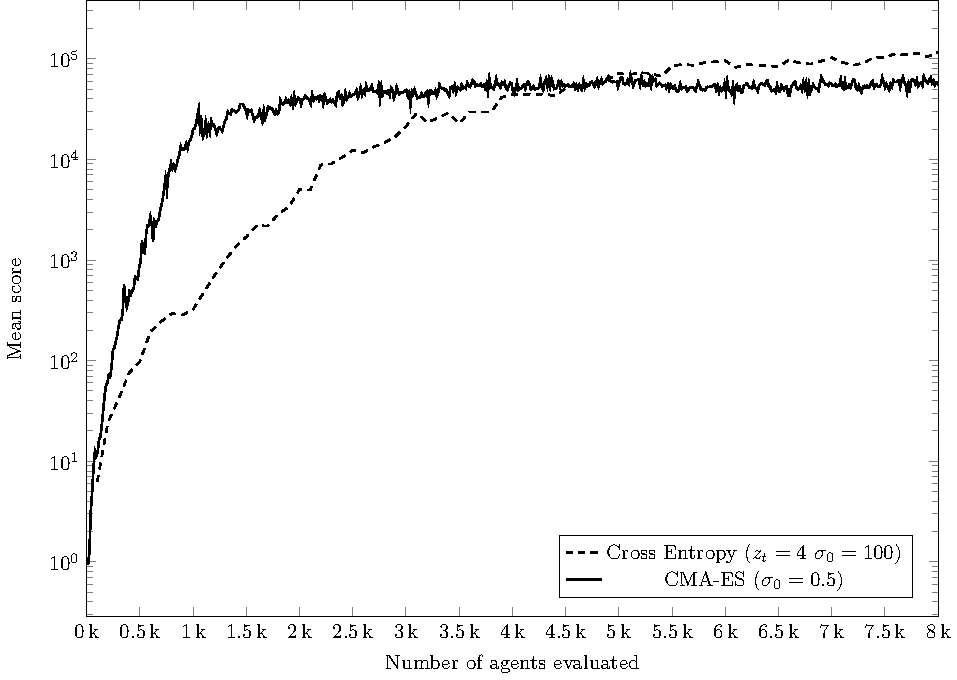
\includegraphics[scale=1]{plots/cmaCePlot}
\caption{Initial comparison between CMA-ES and Cross Entropy \label{fig:CMA_VS_CE_00}}
\end{figure}

As figure \ref{fig:CMA_VS_CE_00} reveals that CMA converges faster,
but reaches a local optimum at around 2,000 games played. Meanwhile CE has a 
slower convergence but reaches a better mean score compared to CM at around 5,500
agents evaluated. In detail, CMA on average reaches a score of 50,000 rows, and
CE reaches a score of 100,000.\\

\comment{Add the raw graphs to appendix}

\textbf{Analysis and discussion}

These results clearly defy our initial hypothesis as we predicted
for CMA to outperform CE, due to its more sophisticated nature. 
One reason for this outcome could possibly be that
CMA has a very little population size compared to Cross Entropy,
which could be a decisive lack as the objective function is noisy with 
a high variance. These results indicate a need to adjust the CMA
configuration, to prevent the too fast convergance.

Among the possible adjustments are:\\
\\
\textit{Enlargment of population size}\\
As the population size is quite small (only around 13)
for this experiment, the CMA algorithm might not be able
extract enough information at each generation. As seen in 
section \ref{optimalsettingsce}, CE looses performance as 
thepopulation size is set too low. This might be a problem 
that counts for CMA as well. In figure \ref{fig:CMA_VS_CE_00},
the CMA algorithm has much the same shape as \\
\\
\textit{Evaluate each agent multiple times}\\
A posible source of poor performance could be 
that the ranking of agents becomes very difficult
due to high noise. To better verify the actual
performance of an agent, it could be evaluated 
multiple times and let the mean of the evaluations
determine it's ranking.\\
\\
\textit{Change the recombination type}\\
As described in section \ref{CMAtheory}, 
the CMA algorithm is not bound to update its 
new mean to just the centroid of the selected 
vectors. Instead, it can weight better solutions
more heavily when moving its mean. When doing so,
it risks biasing vectors that appear to be better 
but in reality, just by faulty ranking, should
not be considered a good agent.\\
\\
None of the experiments seen so far has allowed a 
consistent mean score of more 
than 200,000. This brings concern into 
consideration, that it might be the objective function
that poses a natural limit on the score.
In this case the objective function
models playing Tetris with the Bertsekas featureset. 
It is unkown to us
whether it's possible to construct an agent 
with a mean score of more than
200,000 lines on average. 
Yet, as our aim is not to find the best controller,
untill both algorithms reaches the same upper limit 
of scores theres is no need
to alter the featureset just to
expand the maximum score reachable.\\
\\
Yet, to minimize the likelihood 
that the featureset were the cause of the 
poor performance of CMA, it seemed 
appropiate to conduct a similar comparison 
using another featureset. 
To speed up the process, the game difficulty were 
adujsted to casue agents to fail faster.
The increased difficulty and alternate
featureset is described in 
further detail in section \ref{compoffeatureset}.



\subsubsection{Tuned comparison \label{tunedComparison}}




